%label:"fig:3EndedLagrangianCobordismGammaPlus"
%author:JeffHicks
%name:"3 ended Lagrangian cobordism with curve $\gamma^+$"
%type:"figure"
%parent:exr_biranCornea3ended
%caption:"Profile of the curve $\gamma^+$"


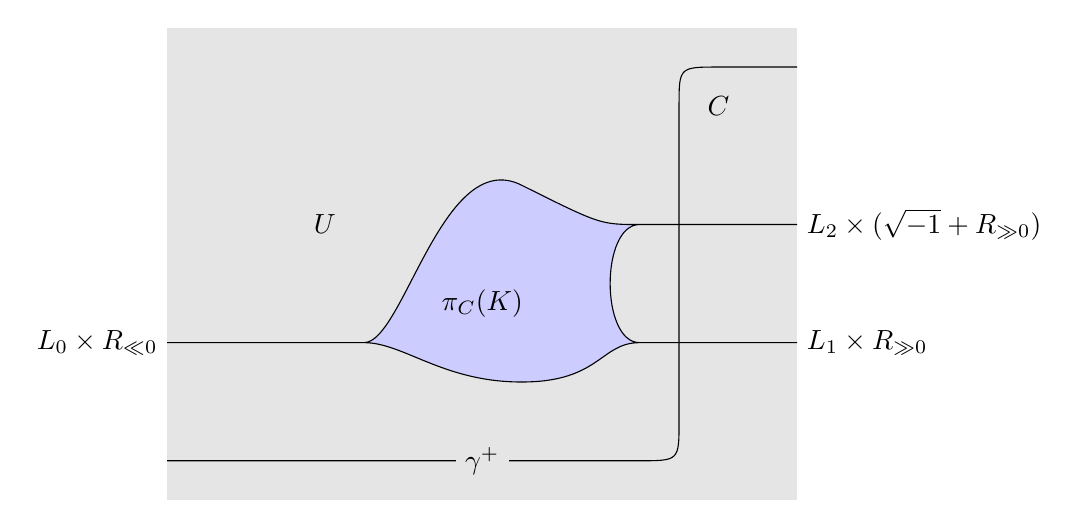
\begin{tikzpicture}

\fill[gray!20]  (-3.5,2.5) rectangle (4.5,-3.5);

\draw[fill=blue!20] (-3.5,-1.5) .. controls (-3,-1.5) and (-1.5,-1.5) .. (-1,-1.5) .. controls (-0.5,-1.5) and (0,-2) .. (1,-2) .. controls (2,-2) and (2,-1.5) .. (2.5,-1.5) .. controls (3,-1.5) and (4,-1.5) .. (4.5,-1.5) .. controls (4,-1.5) and (3,-1.5) .. (2.5,-1.5) .. controls (2,-1.5) and (2,0) .. (2.5,0) .. controls (3,0) and (4,0) .. (4.5,0) .. controls (4,0) and (3,0) .. (2.5,0) .. controls (2,0) and (2,0) ..(1,0.5) .. controls (0,1) and (-0.5,-1.5) .. (-1,-1.5);
\node[left] at (-3.5,-1.5) {$L_0\times \mathbb R_{\ll 0}$};
\node[right] at (4.5,-1.5) {$L_1\times \mathbb R_{\gg 0}$};
\node[right] at (4.5,0) {$L_2\times(\sqrt{-1}+ \mathbb R_{\gg 0})$};
\node at (0.5,-1) {$\pi_{\mathbb C}(K)$};
\node at (3.5,1.5) {$\mathbb C$};
\node at (-1.5,0) {$U$};
\draw (-3.5,-3) .. controls (2,-3) and (2,-3) .. (2.5,-3) .. controls (3,-3) and (3,-3) .. (3,-2.5) .. controls (3,-2) and (3,1) .. (3,1.5) .. controls (3,2) and (3,2) .. (3.5,2) .. controls (4,2) and (4,2) .. (4.5,2);
\node[fill=gray!20] at (0.5,-3) {$\gamma^+$};
\end{tikzpicture}